%%%%%%%%%%%%%%%%%%%%%%%%%%%%%%%%%%%%%%%%%%%%%%%%%%%%%%%%%%%%%%%%%%%%%%%%%%%%%%%%
\fullwidth{\section{Questões xxx}}

\question
Esta é uma questão de múltipla escolha comum.
\begin{choices}
\choice Alternativa errada
\choice Alternativa errada
\choice Alternativa errada
\CorrectChoice Alternativa correta
\choice Alternativa errada
\end{choices}

\question
Esta questão tem um código e múltipla escolha

\begin{tcolorbox}\small
\begin{verbatim}
#include <stdio.h>

int main (void) {
    printf("%d", "Olá, mundo!");
    return 0;
}
\end{verbatim}
\end{tcolorbox}

O que está errado no código?

\begin{choices}
\CorrectChoice Alternativa correta
\choice Alternativa errada
\choice Alternativa errada
\choice Alternativa errada
\choice Alternativa errada
\end{choices}

\question
Esta questão tem uma figura:

\begin{figure}[H]
\centering
\caption{Legenda da figura}
\label{fig:orto1}
\fbox{
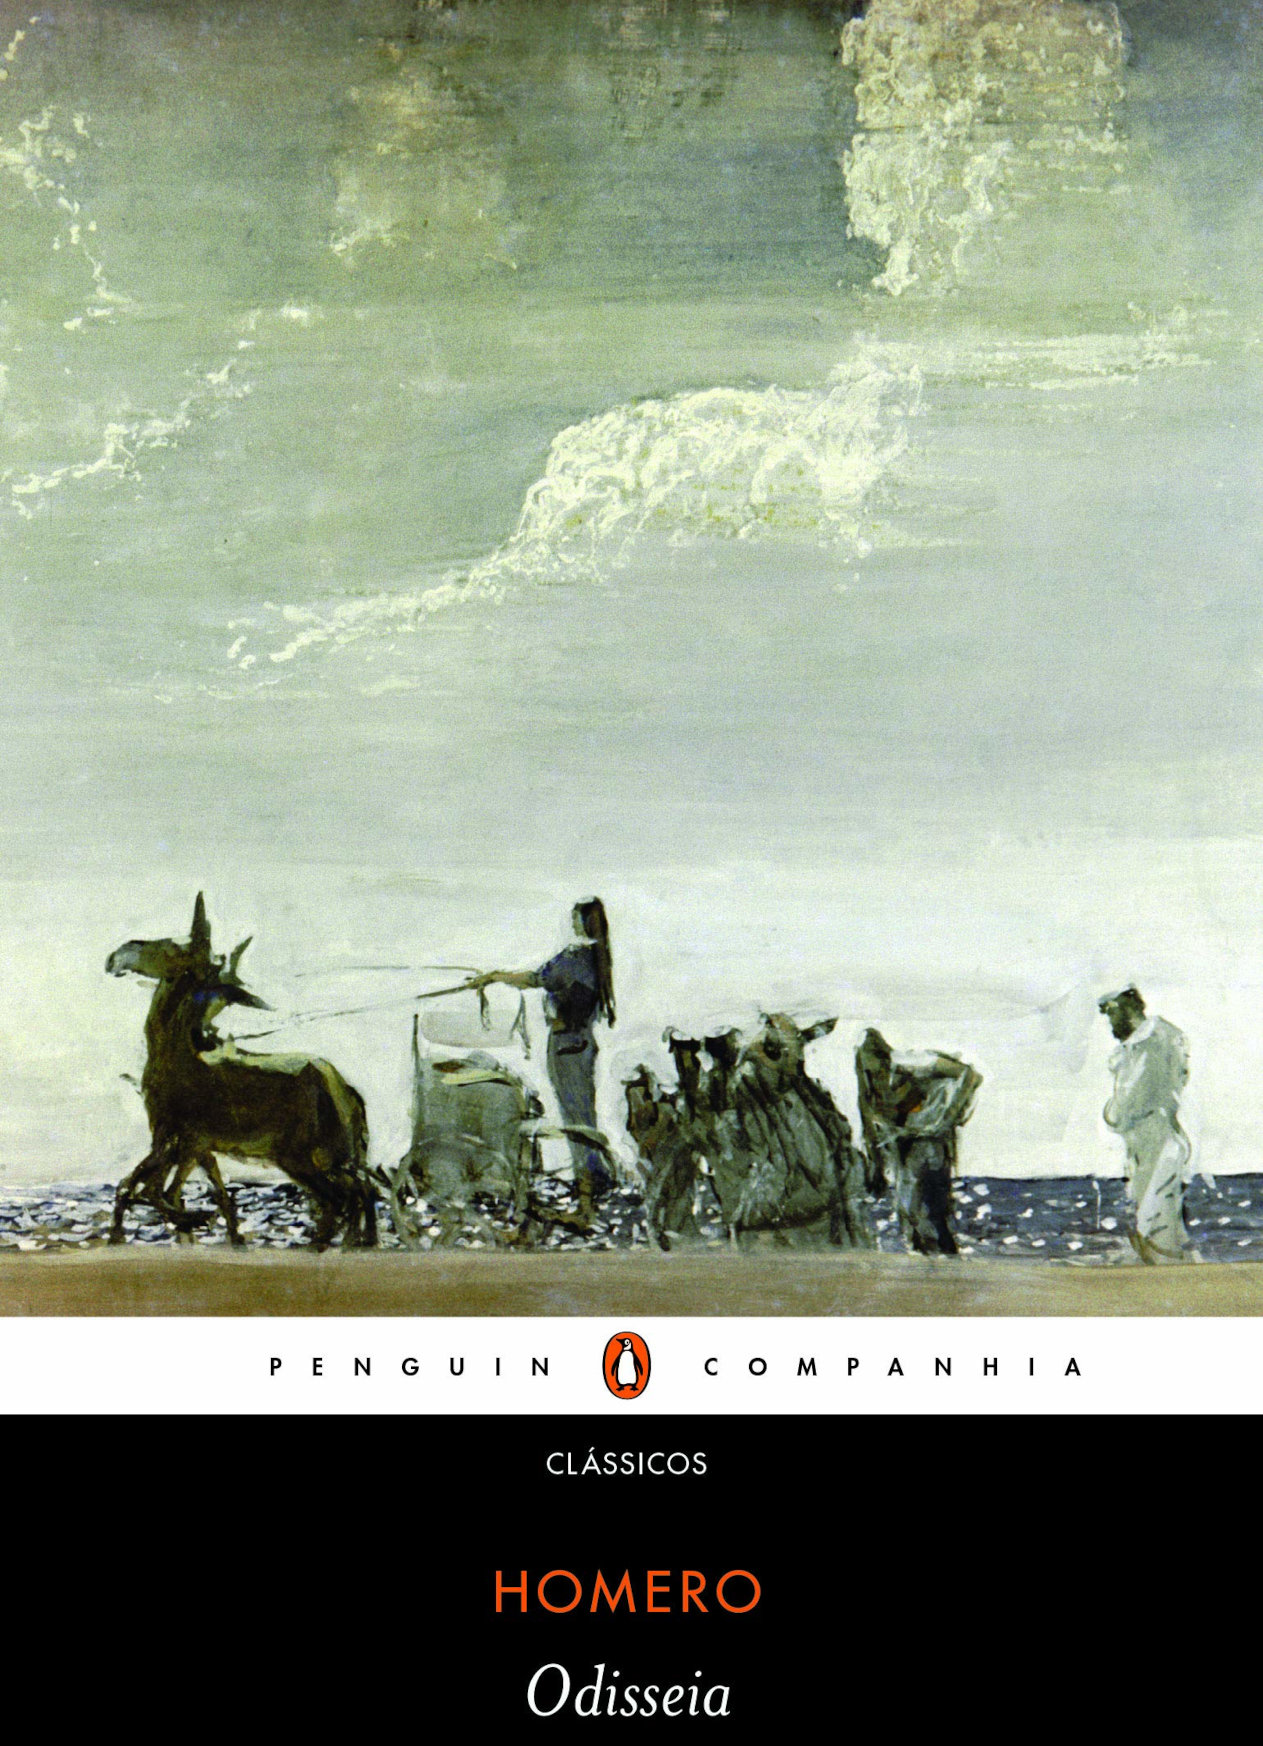
\includegraphics[scale=0.1]{imagens/cover/odisseia2.jpg}
}
\end{figure}

Aqui estão as alternativas:

\begin{choices}
\CorrectChoice Alternativa correta
\choice Alternativa errada
\choice Alternativa errada
\choice Alternativa errada
\choice Alternativa errada
\end{choices}

\question
Esta é uma questão de múltipla escolha em 1 parágrafo:

\hspace{0.92cm}\begin{oneparchoices}
\CorrectChoice XXX
\choice YYY
\choice ZZZ
\choice WWW
\choice TTT
\end{oneparchoices}

\newpage
\question
Esta é uma questão de afirmativas verdadeiras ou falsas.
\begin{itemize}
\item[I.] Afirmativa um.
\item[II.] Afirmativa dois.
\item[III.] Afirmativa três.
\item[IV.] Afirmativa quatro.
\end{itemize}
É correto apenas o que se afirma em:
\begin{choices}
\choice Apenas I
\choice I e IV
\CorrectChoice II e III
\choice Apenas II
\choice Apenas III
\end{choices}

\question
Esta é uma questão discursiva. É verdade que \(x^n + y^n = z^n\) se \(x,y,z\)
e \(n\) são inteiros positivos? Explique.
\treslinhas

\question
Calcule \[\int_{0}^{\infty} \frac{\sin(x)}{x}\]
\vspace{3cm}

\question 
Esta questão tem partes e subpartes. Dada a equação \(x^n + y^n = z^n\) para
\(x,y,z\) e \(n\) inteiros positivos.

\begin{parts}
\part Para quais valores de \(n\) a afirmação na questão é verdadeira?
\duaslinhas

\part Para \(n=2\) existe um teorema com um nome especial. Qual é esse nome?
\umalinha

\part Que famoso matemático fez uma prova elegante desse teorema mas que não
foi escrita pois não havia espaço suficiente na margem do papel?
\umalinha

\begin{subparts}
\subpart Quem realmente provou o teorema?
\umalinha
\subpart Quanto tempo ele levou para resolver o problema?
\umalinha
\end{subparts}

\end{parts}

\newpage
\question
Essa questão é de V ou F:
\begin{parts}
  \part \vf[V] Alternativa verdadeira
  \part \vf[F] Alternativa falsa
\end{parts}

\question
Esta é uma questão do tipo asserção-razão.
Considere as afirmações a seguir, blá, blá, blá:
\begin{itemize}
\item[I.] Aqui está a asserção
          \begin{equation*}
          \text{PORQUE}
          \end{equation*}
          \vspace{-0.8cm}
\item[II.] Aqui está a razão proposta.
\end{itemize}
A respeito dessas afirmações, assinale a alternativa correta:
\begin{choices}
\choice A primeira afirmação é verdadeira e a segunda é falsa.
\CorrectChoice A primeira afirmação é falsa e a segunda é verdadeira.
\choice As duas afirmações são verdadeiras e a segunda é uma justificativa
        correta da primeira.
\choice As duas afirmações são verdadeiras e a segunda não é uma justificativa
        correta da primeira.
\choice As duas afirmações são falsas.
\end{choices}

%%%%%%%%%%%%%%%%%%%%%%%%%%%%%%%%%%%%%%%%%%%%%%%%%%%%%%%%%%%%%%%%%%%%%%%%%%%%%%%%
\fullwidth{\section{Explicações}}

Este modelo de prova utiliza a classe \textbf{exam} para o \LaTeX. Muitos outros
tipos de questões estão disponíveis, bem como diversas configurações para a
contagem de pontuação. Por favor, verifique a documentação em:
\url{https://ctan.org/pkg/exam}.

\question
Um último exemplo de questão discursiva: o que você achou deste modelo?
Lembre-se: a melhor crítica é a \textbf{crítica destrutiva}!
\dezlinhas
